\documentclass[12pt, draft]{article}
\usepackage{candor, setspace, wrapfig}
\newcommand{\BWFtitle}{Computationally Modeling Ribosomal Translation
    and Programmed Frameshifts in}

\usepackage[final, colorlinks=true, linkcolor=BWFBlue,
  citecolor=BWFGreen, urlcolor=BWFRed, pdftitle={\BWFtitle Escherichia coli},
  pdfauthor={Hao Lian, Vivek Bhattacharya, and Daniel Vitek},
  pdfsubject={Bioinformatics, Genetics, and Biology}, pdfcreator={The
    Frameshift Kids}, pdfkeywords={bioinformatics,genetics,biology,
    frameshifts,perl,matlab,ecoli,prfb,rpos,bgh}, pdfstartview={FitH}]{hyperref}

\linespread 2
\numberwithin{equation}{section}

\author{{\sc Hao Lian, Vivek Bhattacharya, and Daniel Vitek}}
\date{{\sc \today}}
\title{\bf{\BWFtitle~\emph{Escherichia coli}}}

\begin{document}
\pagenumbering{roman}
\maketitle
\tableofcontents
\clearpage
\pagenumbering{arabic}

\section{Materials and Methods}
\subsection{Displacement Deviation and Translational Efficiency}


\section{Parameters}
For these plots, we used a species angle of $\theta_{\rm{sp}}
=-30\degree$.

\section{Results}

\subsection{\prfB}

\begin{figure}
  \centering
  \caption{Stochastic displacement plot of \prfB}
  \label{prfB}
  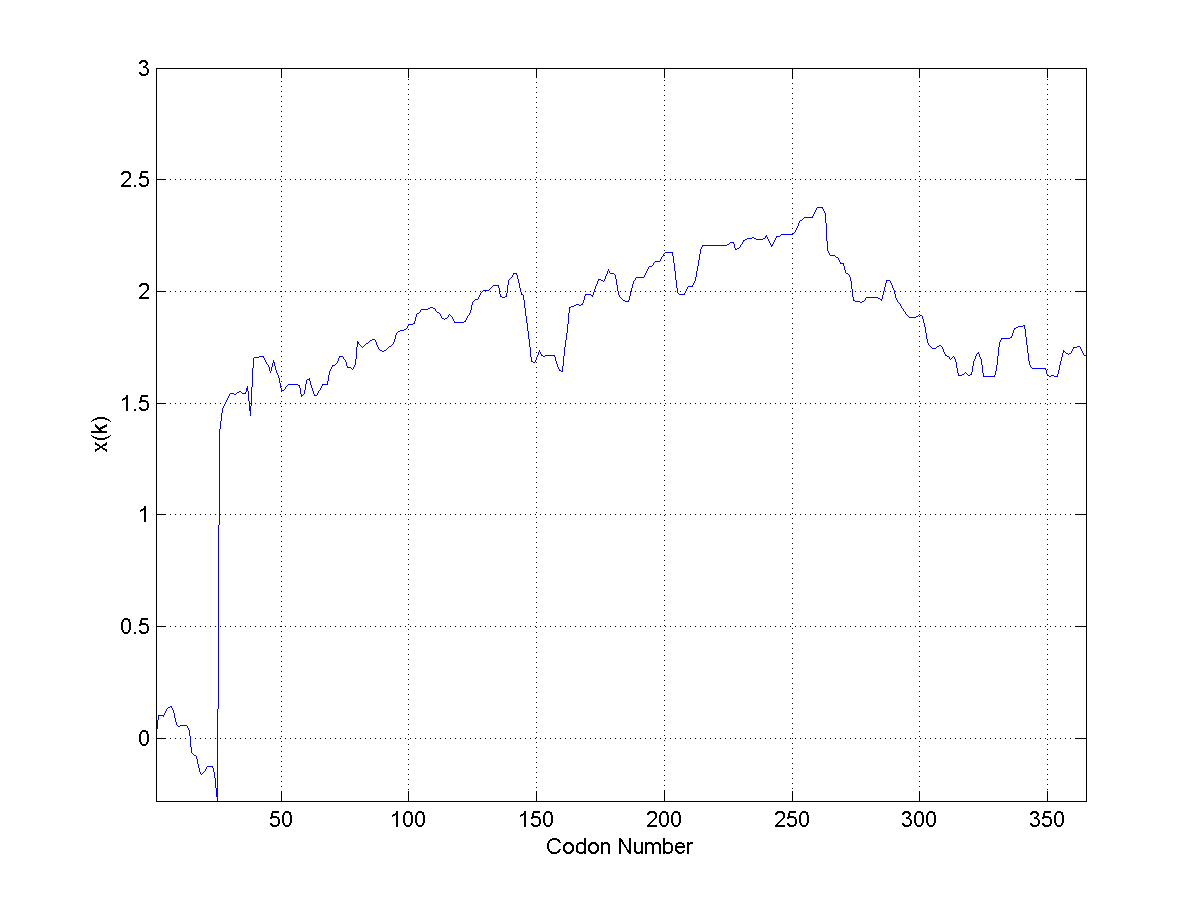
\includegraphics[scale=0.4]{prfB/disp}
\end{figure}

In \ecoli, the gene \prfB\ codes for protein release factor B, an
essential element in translation.  This gene, as mentioned, is known
to have a programmed frameshift at the 25$^{\textrm{th}}$ codon.
\autoref{prfB} shows a displacement plot for
\prfB, again with a distinctive jump at codon 25.
\footnote{Note that the polar plot is the the same as \autoref{prfB:polar}. 
The new model does not alter the polar plot or the free energy calculations.}

Notably, the displacement plot does not reach $x=2$ over the span of one codon, as the old model predicted.
Rather, due to randomness, the ribosome chooses the codon in the $+1$ frame before actually reaching a displacement of exactly 2.
The propensity to approach $x=2$, however, concurs with biological
evidence indicating the ribosome stays in frame after the frameshift.
[Dr. Stomp, we need references here.]

\begin{figure}
  \centering
  \caption{Sensitivity plot for \prfB}
  \label{prfB:sens}
  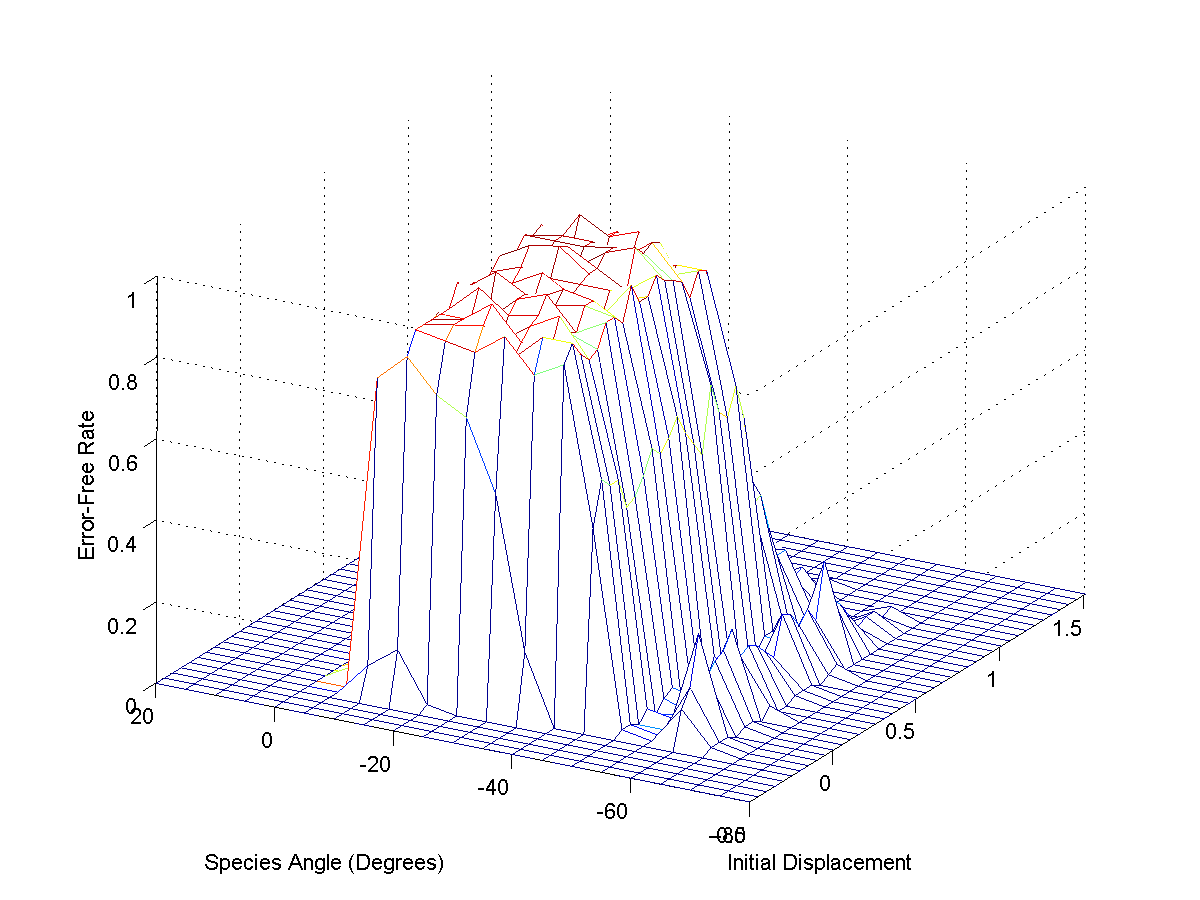
\includegraphics[scale=0.4]{prfB/sensitivity}
\end{figure}

 We repeated Weiss's experiments computationally
using the stochastic model, and our results agreed~\cite{weiss87,weiss88}.
This concurrence again provides support for the biological validity of
the stochastic model.

Specifically, \citeauthor{weiss87} moved the stop codon in the
\prfB\ sequence one nucleotide upstream, causing the sequence to fail to
frameshift. Moving the stop codon another nucleotide upstream failed
to create a frameshift as well in our model.

\subsection{\ecoli\ genes}

\begin{wrapfigure}{R}{0.55\textwidth}
  \centering
  \caption{Displacement deviation for \ecoli\ genes with with
    deviation >3 (<1\%) truncated}
  \label{ecoli:hist}
  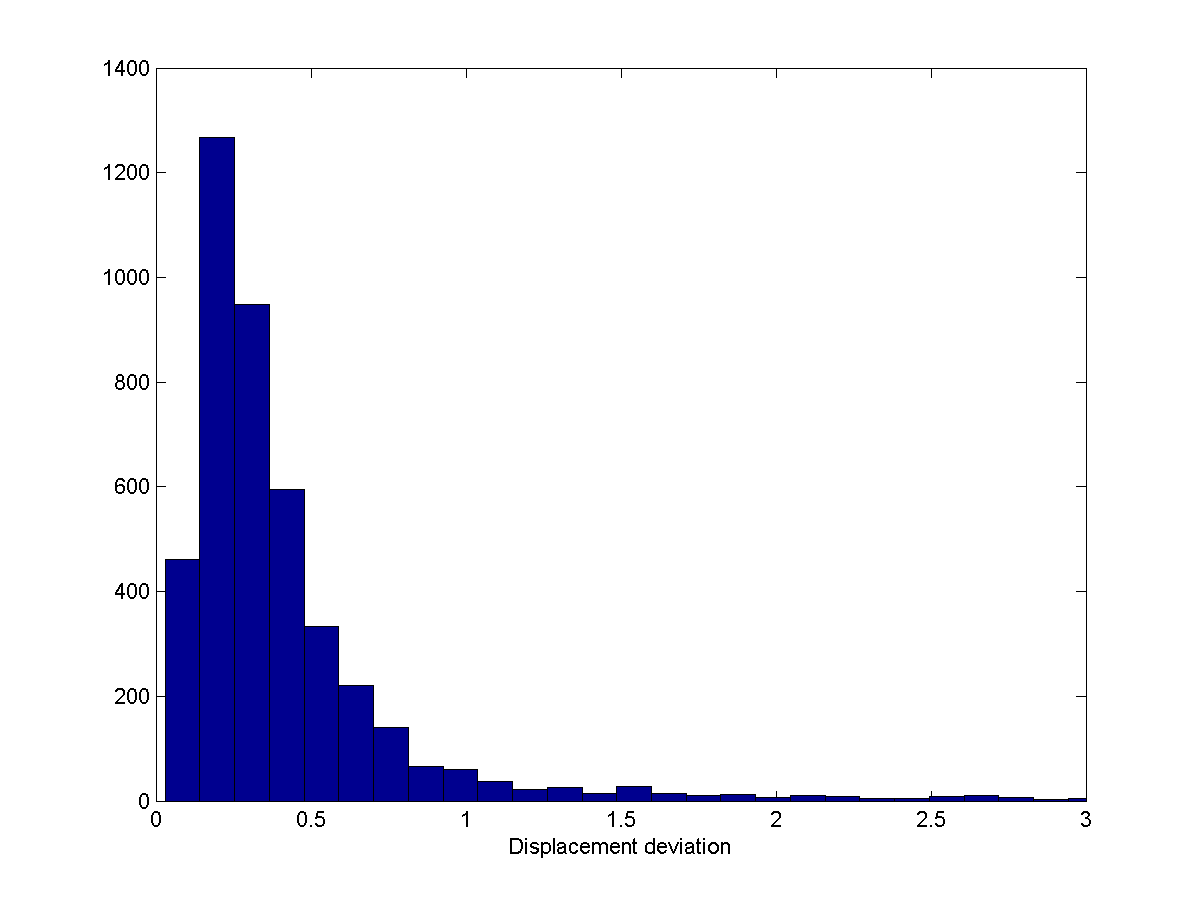
\includegraphics[width=0.55\textwidth]{histograms/everything}
\end{wrapfigure}

\ecoli, as a product of evolution, is naturally efficient in its
processes. [Dr. Stomp, we need references here.]
It logically follows that the model should indicate low deviation
for most \ecoli\ proteins.
\autoref{ecoli:hist} is a histogram of the deviation yields of 4364 genes of
\ecoli, over 80\% of the entire genome.  As predicted, 93.45\% of the genes that we ran
[Guys, expand on this.] laid in the 0 to 1 interval.  The average displacement deviation
for these \ecoli\ genes is [Guys, what?], in a run for 100 iterations per genes.

\subsection{Ribosomal Proteins}
To compound this finding, biologists also agree that ribosomal
proteins offer especially high translational efficiencies, since the
cell must produce them in such large quantities. [Dr. Stomp, we need
  references here.] The displacement deviation for ribosomal proteins
is in fact [Guys, what?]. We found the average displacement deviation
to be [Guys, what?], which is significantly lower with a $t$-value of
[Guys, what?].

[Guys, outliers.]

\subsection{Bovine Growth Hormone}
\label{section:bgh}

We investigated the concept of deviation yield as a measure of biological
yield by studying bovine growth hormone (bGH), a protein commonly used
in agriculture.
Research~\cite{schoner:bgh} at the time attempted to produce bGH
in \ecoli\ in large amounts.

\begin{tabular}{lccc}
  \toprule
  \textbf{Sequence} & $d$ & $\sigma(d)$ & Yield (\% bGH)\\
  \midrule
  pCZ101 & 0.5146 & 0.03313 & 30 \\
  pCZ105 & 0.5139 & 0.04181 & 34\\
  pCZ112 & 0.6612 & 0.03633 & 33\\
  pCZ115 & 0.6721 & 0.03792 & 32\\
  \midrule
  pCZ100 & 0.7107 & 0.01715 & $<$ 0.5\\
  pCZ104 & 0.7162 & 0.01433 & $<$ 0.5\\
  pCZ108 & 0.5912 & 0.05976 & 1.7\\
  pCZ110 & 0.7026 & 0.01966 & $<$ 0.5\\
  \bottomrule
\end{tabular}


\citet{schoner:bgh}, primarily modifying the initial codons of an
initial bovine growth hormone sequence, found sequences pcZ101,
pcZ105, pcZ112, and pcZ115, to have particularly high protein yield
and to be efficient in comparison to the six other sequences. In
modeling displacement, we found these four sequences  to have the least
displacement deviation from $x = 0$
(\autoref{bgh:deviation}). \autoref{bgh:disp} shows the displacement
plots of all the bGH sequences on the same set of axes. Although not
immediately obvious, the four sequences do indeed indicate lower
deviation. Despite running the genetic algorithm, pcZ108 remains an
outlier because \citeauthor{schoner:bgh} reported low protein
efficiency whereas our model reports low deviation, incongrous with
previously established correlations.

\begin{figure}
  \centering
  \caption{Displacement plot for bGH}
  \label{bgh:disp}
  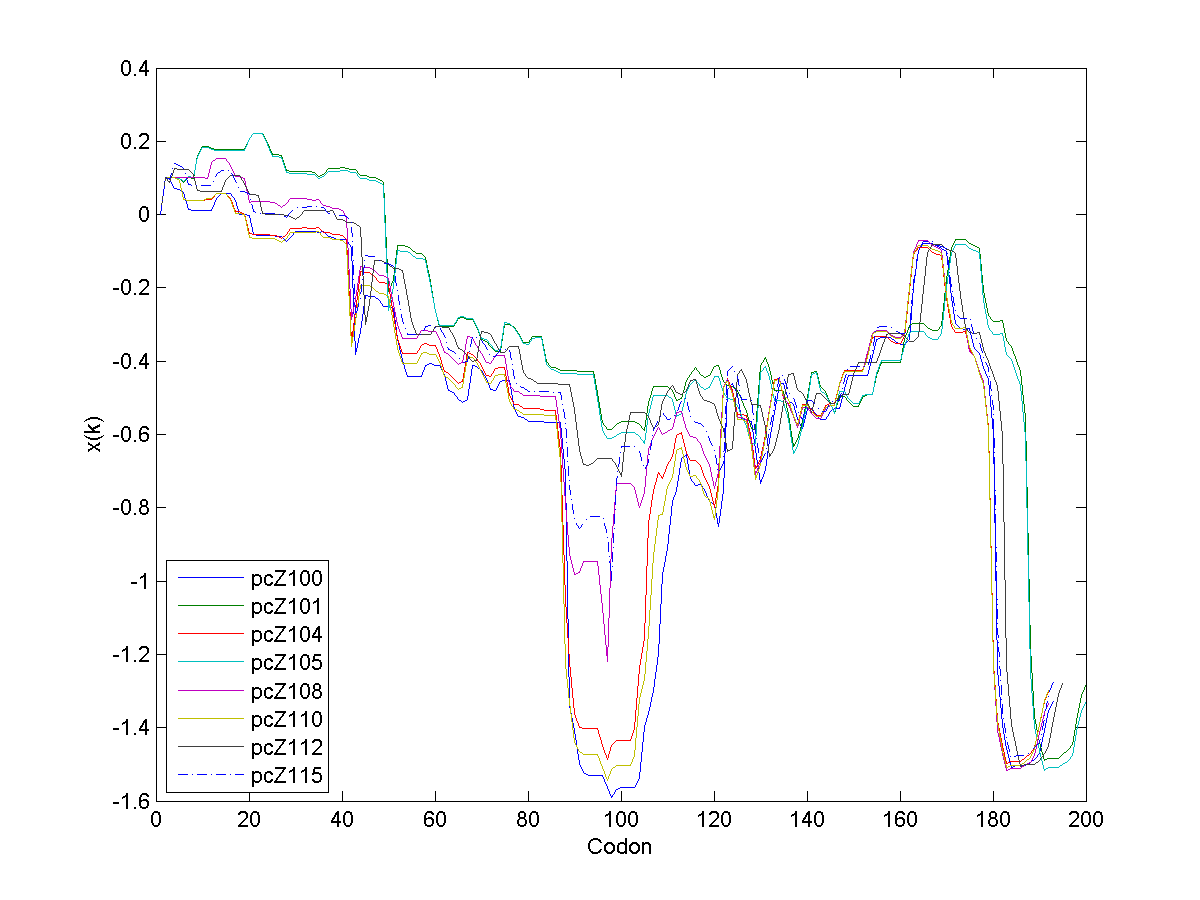
\includegraphics[scale=0.4]{bgh/all}
\end{figure}

\subsection{Optimizing Translational Efficiency}

If deviation yield is in fact a potential metric for biological yield,
a method for optimizing deviation would be of use of biologists.  As such,
we wrote an algorithm to minimize deviation for given sequences.
We tested this algorithm computationally on \rpoS, a gene known to
be translationally regulated.  Biological experiments will be
conducted soon.

% I'm colluding deviation and probability yield here, but it's for a
% good purpose. --Hao.

\citet{rpoS:process} indicate that \rpoS, a gene that codes for an RNA
polymerase sigma factor, contains sections of rare codons that disrupt
ribosomal translation. Indeed, our computation model agrees with this
biological evidence, showing again moderately high deviation from $x =
0$. In mass production of such a polymerase sigma factor, biologists
can replace sequences of codons known to add noise and error to
ribosomal translation with synonymous codons. 
However, with a computation model, the process is much
faster and, with this performance, we can perform a randomized, greedy
algorithmic search for codon sequence replacements. We first find an
early trouble spot\footnote{Specifically, places with
  mistake frameshifts in our model, which correlate to rare codons per
  above discussion.} of four codons, randomly replacing that sequence
with synonymous four codons, and running our model against those
permutations to obtain a locally optimal sequence at that place. We
then repeat for all trouble spots the first, terminating when we have locally
optimized the last one. With this algorithm, we reduced our standard
deviation metric for the \rpoS\ displacement plot from 0.168 to 0.117
on sample size of 1000 with a replacement of 33 codons. The
initial correlation between deviation and biological expression
provides strong anecdotal evidence that, with future biological
experimentation, our algorithm has indeed increased protein yield
bypassing a potentially slow biological experimentation process.

[Dr. Stomp, we need the notes that you mentioned.]

\section{Discussion}
Yet, we must note that the model is quite robust; minor changes
in $\theta_{\rm{sp}}$ and initial displacement do not affect frameshifting significantly~\autoref{prfB:sens}.
\autoref{prfB:sens} illustrates the error-free rate as
a function of species angle and initial displacement. As noted,
the frameshift holds over quite a wide range.

Therefore, our model agrees with life in that ribosomal proteins
express much more highly than genes in general.

These results from bovine growth hormone in addition to correlation with a broad
spectrum of known ribosomal behavior indicate our computational model
can significantly increase the speed at which geneticists and
biologists can obtain valuable information when synthesizing
commercially or medicinally useful compounds without laboriously
working through biological experiments.

Our model agrees with his findings.

\phantomsection
\addcontentsline{toc}{section}{References}
\begin{singlespace}
  \bibliography{wizards}
\end{singlespace}
\end{document}
